\par{Table \ref{tab:xeon_arch} contains the main hardware characteristics of the
    Xeon CPU installed in fionn.}

\begin{table}[!h]
    \centering
    \begin{tabular}{| l | l | l | l |}
    \hline
    \# cores / socket& 10(out-of-order) \\ \hline
    \# threads / core& 2 \\ \hline
    \# sockets & 2 \\ \hline
    clock speed & 2.2 GHz \\ \hline
    typr & Ivy Bridge \\ \hline
    vector unit & 256-bit AVX \\ \hline
    L1 / core & 32KB(data)+32KB(instructions) 64KB total \\ \hline
    L2 / core & 256KB \\ \hline
    L3 /socket & 25MB \\ \hline
    \end{tabular}
    \caption{Xeon characteristics\cite{xeon_specs}.}
    \label{tab:xeon_arch}
\end{table}

\subsubsection{Mapping}

\par{The mapping of OpenCL concepts to Hardware are the same that in the Xeon 
    Phi, see section \ref{sec:phi}. Figure \ref{XeonDi} shows the capabilities of 
    the unerlying hardware found by OpenCL queries.}

\begin{figure}[!h]
    \centering
    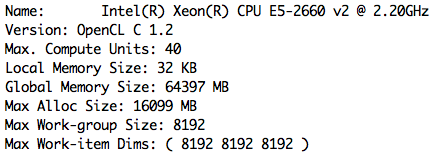
\includegraphics[width=0.49\textwidth]{figures/xeon_di.png}
    \caption{Xeon Device Information.}
    \label{XeonDi}
\end{figure}

